\documentclass[twoside]{article}
\setlength{\oddsidemargin}{-0.5 in}
\setlength{\evensidemargin}{1.5 in}
\setlength{\topmargin}{-0.6 in}
\setlength{\textwidth}{5.5 in}
\setlength{\textheight}{8.5 in}
\setlength{\headsep}{0.5 in}
\setlength{\parindent}{0 in}
\setlength{\parskip}{0.07 in}
\setlength{\marginparwidth}{145pt}

%
% ADD PACKAGES here:
% 12

\usepackage{amsmath,
            amsfonts,
            amssymb,
            graphicx,
            mathtools,
            flexisym,
            marginnote,
            hyperref,
            titlesec}

\usepackage[english]{babel}
\usepackage[utf8]{inputenc}
\usepackage[shortlabels]{enumitem}

\graphicspath{ {images/} }

\hypersetup{
    colorlinks=true,
    linkcolor=blue,
    filecolor=magenta,      
    urlcolor=blue,
}

\titlespacing\section{0pt}{12pt plus 4pt minus 2pt}{0pt plus 2pt minus 2pt}
\titlespacing\subsection{0pt}{12pt plus 4pt minus 2pt}{0pt plus 2pt minus 2pt}

%
% The following commands set up the lecnum (lecture number)
% counter and make various numbering schemes work relative
% to the lecture number.
%
\newcounter{lecnum}
\renewcommand{\thepage}{\thelecnum-\arabic{page}}
\renewcommand{\thesection}{\thelecnum.\arabic{section}}
\renewcommand{\theequation}{\thelecnum.\arabic{equation}}
\renewcommand{\thefigure}{\thelecnum.\arabic{figure}}
\renewcommand{\thetable}{\thelecnum.\arabic{table}}

\newcommand{\aosv}{1044414: Advanced Operating Systems and Virtualization}
\newcommand{\wir}{1038137: Web Information Retrieval}
\newcommand{\va}{1052057: Visual Analytics}
\newcommand{\advprog}{1044416: Advanced Programming}
\newcommand{\dchpc}{1044399: Data Centers and High Perf. Computing}

\newcommand{\qu}[1]{\marginnote{\textcolor{cyan}{#1}}}


%
% The following macro is used to generate the header.
%
\newcommand{\lecture}[4]{
   \pagestyle{myheadings}
   \thispagestyle{plain}
   \newpage
   \setcounter{lecnum}{#4}
   \setcounter{page}{1}
   \noindent
   \begin{center}
   \framebox{
      \vbox{\vspace{2mm}
    \hbox to 7.4in { {\bf #1
    \hfill Spring 2018} }
       \vspace{4mm}
       \hbox to 7.4in { {\Large \hfill Lecture #4: #2  \hfill} }
       \vspace{2mm}
       \hbox to 7.4in { {\it Lecturer: #3 \hfill Scribe: Anxhelo Xhebraj} }
      \vspace{2mm}}
   }
   \end{center}
   \markboth{Lecture #4: #2}{Lecture #4: #2}

   \iffalse
   {\bf Note}: {\it LaTeX template courtesy of UC Berkeley EECS dept.}

   {\bf Disclaimer}: {\it These notes have not been subjected to the
   usual scrutiny reserved for formal publications.  They may be distributed
   outside this class only with the permission of the Instructor.}
   \vspace*{4mm}
   \fi
}
%
% Convention for citations is authors' initials followed by the year.
% For example, to cite a paper by Leighton and Maggs you would type
% \cite{LM89}, and to cite a paper by Strassen you would type \cite{S69}.
% (To avoid bibliography problems, for now we redefine the \cite command.)
% Also commands that create a suitable format for the reference list.
\iffalse
\renewcommand{\cite}[1]{[#1]}
\def\beginrefs{\begin{list}%
        {[\arabic{equation}]}{\usecounter{equation}
         \setlength{\leftmargin}{2.0truecm}\setlength{\labelsep}{0.4truecm}%
         \setlength{\labelwidth}{1.6truecm}}}
\def\endrefs{\end{list}}
\def\bibentry#1{\item[\hbox{[#1]}]}
\fi

%Use this command for a figure; it puts a figure in wherever you want it.
%usage: \fig{NUMBER}{SPACE-IN-INCHES}{CAPTION}
\newcommand{\fig}[3]{
            \vspace{#2}
            \begin{center}
            Figure \thelecnum.#1:~#3
            \end{center}
    }
% Use these for theorems, lemmas, proofs, etc.
\newtheorem{theorem}{Theorem}[lecnum]
\newtheorem{lemma}[theorem]{Lemma}
\newtheorem{proposition}[theorem]{Proposition}
\newtheorem{claim}[theorem]{Claim}
\newtheorem{corollary}[theorem]{Corollary}
\newtheorem{definition}[theorem]{Definition}
\newenvironment{proof}{{\bf Proof:}}{\hfill\rule{2mm}{2mm}}

% **** IF YOU WANT TO DEFINE ADDITIONAL MACROS FOR YOURSELF, PUT THEM HERE:

\newcommand\E{\mathbb{E}}

\begin{document}

\nocite{*}

%FILL IN THE RIGHT INFO.
%\lecture{**LECTURE-NUMBER**}{**DATE**}{**LECTURER**}{**SCRIBE**}

\lecture{\aosv}{March 9}{Alessandro Pellegrini}{3}

%\footnotetext{These notes are partially based on those of Nigel Mansell.}

% **** YOUR NOTES GO HERE:

\iffalse

\subsection{Task State Segment (continued...)}

The interest part of TSS is the fact that there is one stack segment and pointer for each privilege level. TSS is not accessible in user mode (DPL 0).

The code executes at either code 0 or 3 (kernel mode or user mode). On memory access we trigger a trap that indicates a INterrupt-gate descriptor in the IDT that selects a code segment with DPL 0 and the Gate has DPL 3. The example shown is about software interrupt. The DPL gate should be 3 in order to access code in privilege level 0. The destination code segment is then loaded in the code segment register.

\fi

In the previous lectures we described some processor architecture details that must be setup in order for a kernel to boot and work properly such as protected mode, IDT, GDT etc. In the next lecture we will see the code that initializes and configures such state in the Linux kernel but first we must introduce hardware paging and x64 long mode. \textit{Hardware Paging} is the mechanism through which Linear Adresses are mapped to Physical Addresses by the CPU and should not be confused with paging and memory management in higher abstraction levels (e.g. kernel). In this section Linear Address and Logical Address will be used interchangeably since most OSes use the Flat Model described in the previous lecture making the two coincide.

\iffalse
The difference between Logical, Virtual, Linear, Physical memory:

Logical Address Space: a process memory address before passing through the segmentation unit
Linear Address Space: a process memory address after passing through the segmentation unit but before passing through the paging unit. Coincides with logical address space if flat model
Virtual Memory: a Linear address that is currently not mapped to main memory but maybe stored in disk pp. 151 Vol 3A Intel manual. 
Physical Memory: the "hardware" address that passes in the address bus after segmentation and paging.
\fi

\section{Protected Mode Paging}

Segmented memory in processors' architecture was later coupled with a finer grained memory access by introducing the Paging Unit. This new layer in address translation brings in new memory protection mechanisms which check the requested access type against the access rights of the Linear Address and, if the memory access is not valid, generates a Page Fault exception.

When a Logical Address, the one displayed in debuggers and the one used as displacement in programs, is fed to the processor using some instruction (\texttt{jmp}, \texttt{mov} etc.) it gets mapped to a physical address in RAM through the following steps: it is first translated into a Linear Address by the Segmentation Unit (but as we saw in the previous lectures, by the means of the Flat Model, Logical and Linear Addresses coincide) and then mapped to a Physical Address by the Paging Unit.

\begin{center}
  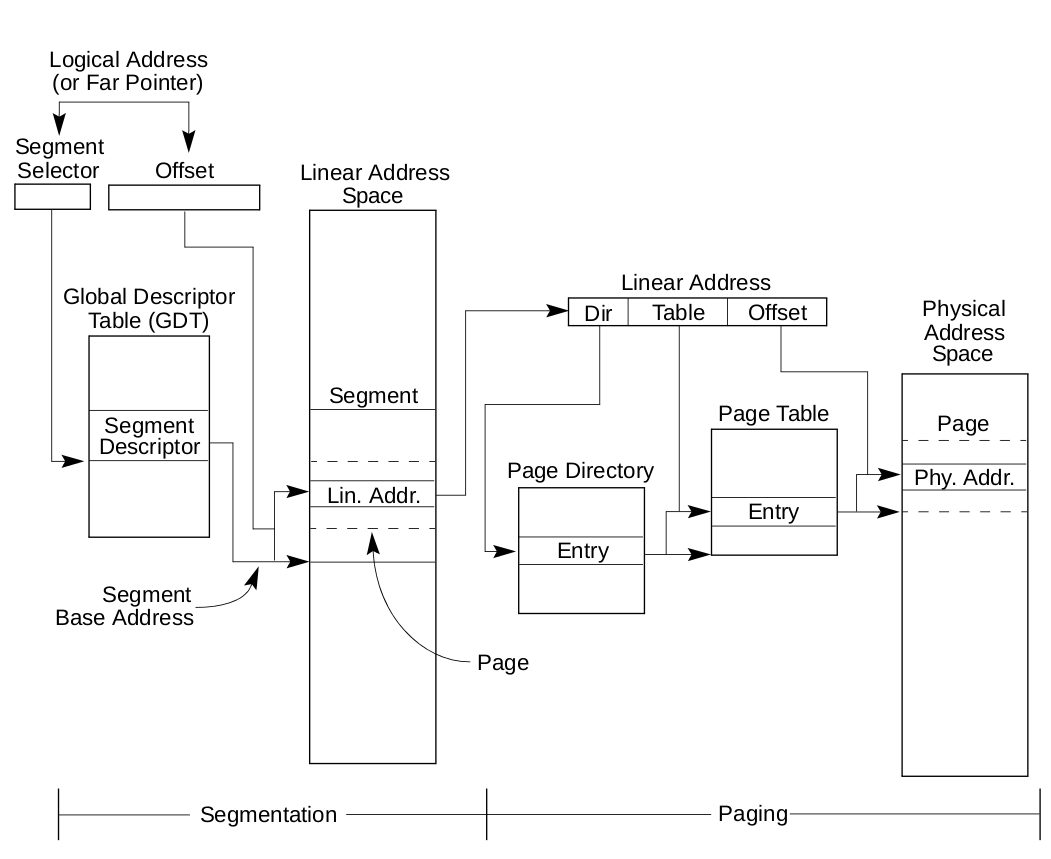
\includegraphics[width=0.6\textwidth]{segpag.png}
  \fig{1}{0 pt}{Logical to Physical Address (\cite{intel} pp. 90) }
\end{center}

The paging unit thinks of all RAM as partitioned into fixed-length \textit{page frames}. Each page frame contains a page which is the data contained in a fixed-length interval of Linear Addresses. Page frames and pages coincide in size.

The CPU needs some data structures stored in main memory called \textit{page tables} to be setup in order to enable paging. Page tables have a hierarchical structure constituted of multiple levels depending on the size of page frames and addressable memory. \marginnote{Page tables are setup by the kernel for each process in the system and managed in order to not overlap on Physical Addresses. This is why multiple instances of the same program refer to same Logical Addresses but do not interfer with each other}[-12pt]

The Physical Address of the first level of the page tables in the hierarchy is stored in the \texttt{CR3} register introduced specifically for paging. \texttt{CR3} must keep the physical address instead of the Logical one because otherwise we would end up in a recursive problem: in order to translate a Logical Address we would have to translate a Logical Address. Whenever the OS needs to change the contents of \texttt{CR3} it has to do so in a careful manner by translating \textit{software side} Logical Addresses to Physical Addresses through its relative position since after protected mode is enabled every address pass through the translation in the MMU.

\subsection{i386 Paging}

The first paging scheme was introduced in the Intel 80386 32-bit processor that handled 4KB pages. The first level page table is called \textit{Page Directory} and the address of the one in use is stored in the \texttt{CR3} register. This table holds Page Directory Entries (PDE). The second level page table is called \textit{Page Table} and holds the Page Table Entries (PTE).

The aim of this two-level scheme is to reduce the amount of RAM required for per-
process Page Tables. \marginnote{With one level we would have to initialise a table of $2^{20}$ entries with 4 Bytes per entry would be 4MB in RAM just for the table}

The 32 bits of a Linear Address are divided into three fields:
\begin{description}
  \itemsep-2pt
  \item [Directory] \texttt{bit[31:22]} determines the entry in the Page Directory that points to the proper Page Table
  \item [Table] \texttt{bit[21:12]} determines the entry in the Page Table that contains the physical address of the page frame containing the page
  \item [Offset] \texttt{bit[11:0]} determines the relative position within the page frame
\end{description}

\marginnote{
  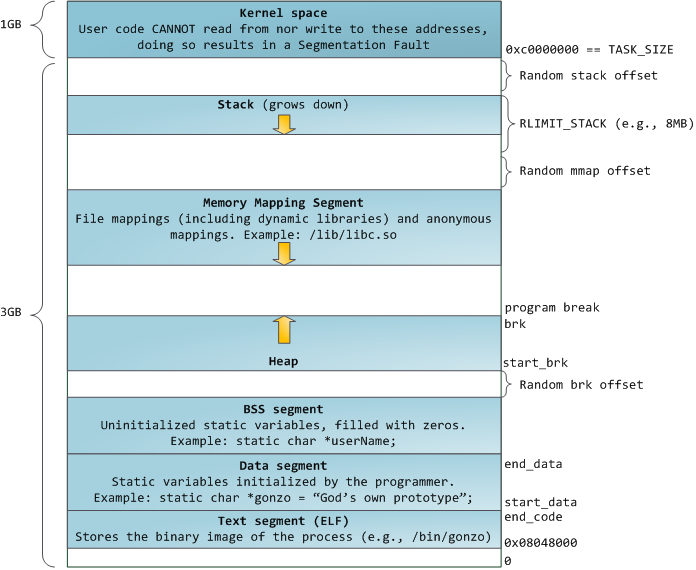
\includegraphics[width=0.5\textwidth]{lini386.png}
  \fig{2}{0 pt}{i386 Linux Process Logical Address Map}
}

\begin{center}
  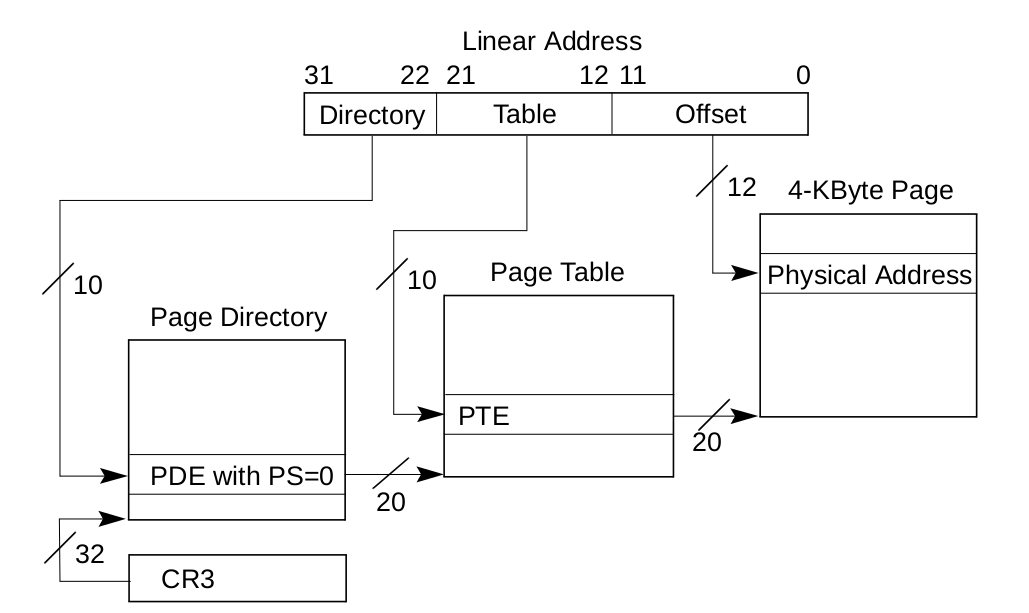
\includegraphics[width=0.6\textwidth]{basicpag.png}
  \fig{3}{0 pt}{i386 Paging Scheme (\cite{intel} pp. 113) }
\end{center}

By the fact that the Offset field is 12 bits long we are able to address each byte of the 4KB page ($2^{12} = $4KB). Also, since each PTE and PDE is of size 4 bytes, 4KB/4B = 1024 PTE or PDE fit in one page therefore the 10 bits of the Table or Directory fields are sufficient to address each PTE or PDE within a Page Directory or Page Table page. From the observations above it follows that this scheme with one Page Directory (4KB in size, only first level) can address up to 1K $\times$ 1K $\times$ 4KB = 4GB.

\marginnote{
  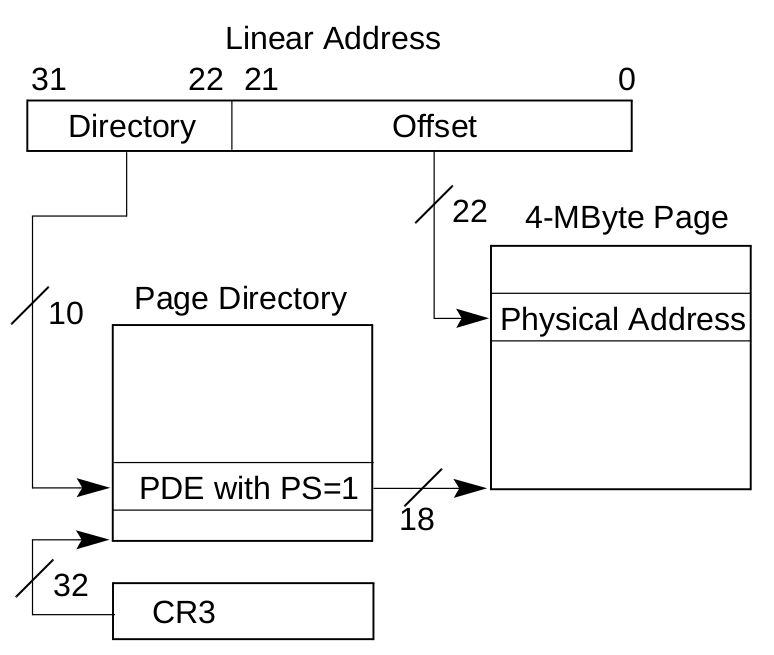
\includegraphics[width=0.4\textwidth]{4MB32.png}
  \fig{5}{0 pt}{4MB pages Physical Address Resolution (\cite{intel} pp. 113) }
}[-2.5cm]

\subsection{PDE and PTE fields}

\iffalse
In this subsection both PDE and PTE are described together. Be careful while reading
\fi

\begin{center}
  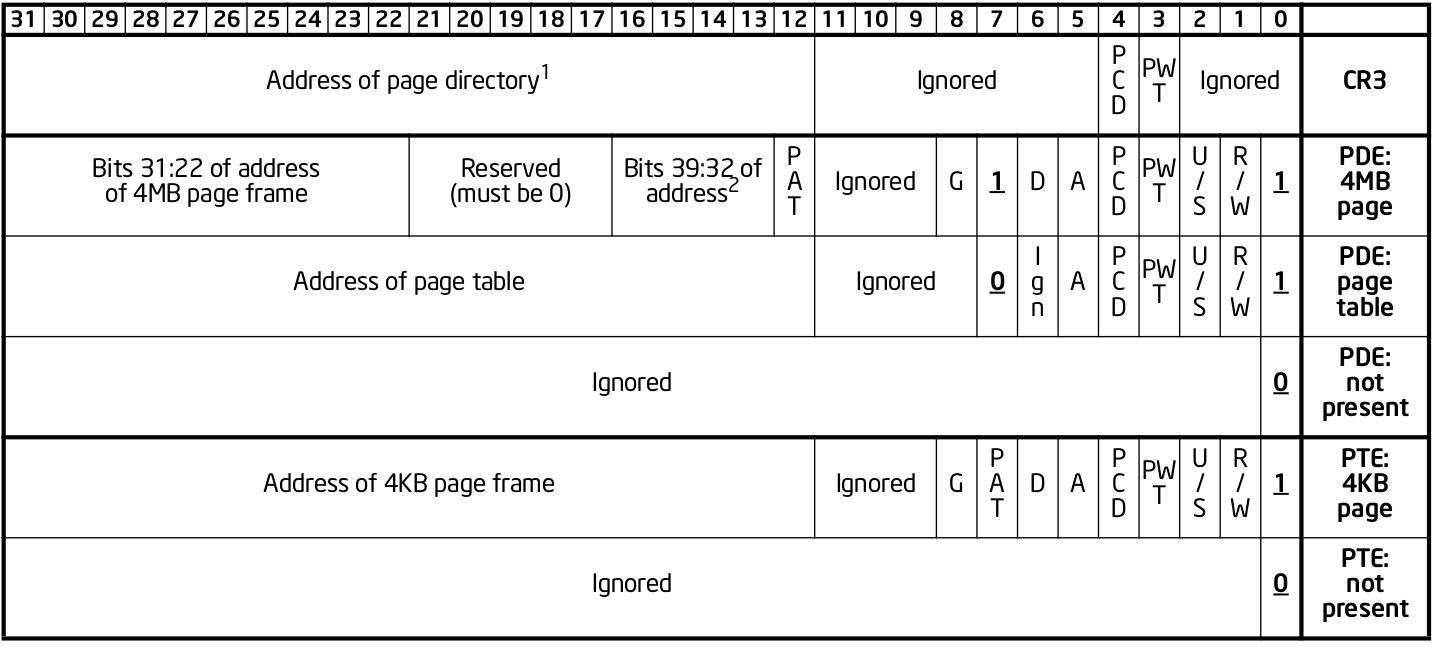
\includegraphics[width=0.8\textwidth]{i386pag.png}
  \fig{4}{0 pt}{PDE and PTE interpretations (\cite{intel} pp. 114) }
\end{center}

\begin{description}
  \itemsep-3pt
  \item [P] Present \marginnote{(\cite{bovet_cesati_2006} pp. 48, \cite{intel} pp. 114-115)}[-24pt] flag: in Page Table must be 1 to map a 4KB page, in Page Directory must be 1 to reference a page table
  \item [R/W] \marginnote{R/W is used for Copy On Write (COW), mechanism to not setup process memory in case of a \texttt{fork()} until changes to variables are performed} Read/Write flag: if 0 writes may not be allowed in the 4KB referenced by a PTE or in all the pages pointed by the Page Table pointed by the PDE (1024 $\times$ 4KB = 4MB region controlled by the PDE)
  \item [U/S] User/Supervisor flag: if 0 user-mode accesses are not allowed to the 4MB region controlled by the PDE or the 4KB referenced by the PTE
  \item [PCD and PWT] Page-level Cache Disable and Page-level Write Through flags: determine the memory type used to access the Page Table referenced by the PDE or the 4KB page referenced by the PTE
  \item[A] \marginnote{ P was used especially on systems having less than 4GB of RAM: processes could Logically Address up to 4GB of memory and this was managed through swapping } Accessed flag: indicates whether the PDE was used for Linear Address Translation or software has accessed the 4KB page referenced by the PTE
  \item[D] Dirty flag: indicates whether the 4KB referenced by the PTE was written by software
  \item[PS] Page Size: in PDE indicates whether the address points to a Page Table or a page of 4MB.  In this case the entry refers to a 4MB page
  \item[G] Global flag: prevents frequently used pages from being flushed from the TLB cache
  \item[Address]: contains the 20 most significant bits of the Physical Address of the page (PTE or PDE with PS=1) or Page Table (in case of PDE with PS=0). Since pages are of 4KB starting from address 0 we need only 20 bits to address all of the 4GB (4KB $\times 2^{20}$ = 4GB)
\end{description}

For further information about the flags and a more detailed explanation we refer the reader to the Intel Manual \cite{intel}.

\subsection{Physical Address Extension (PAE)}

\begin{center}
  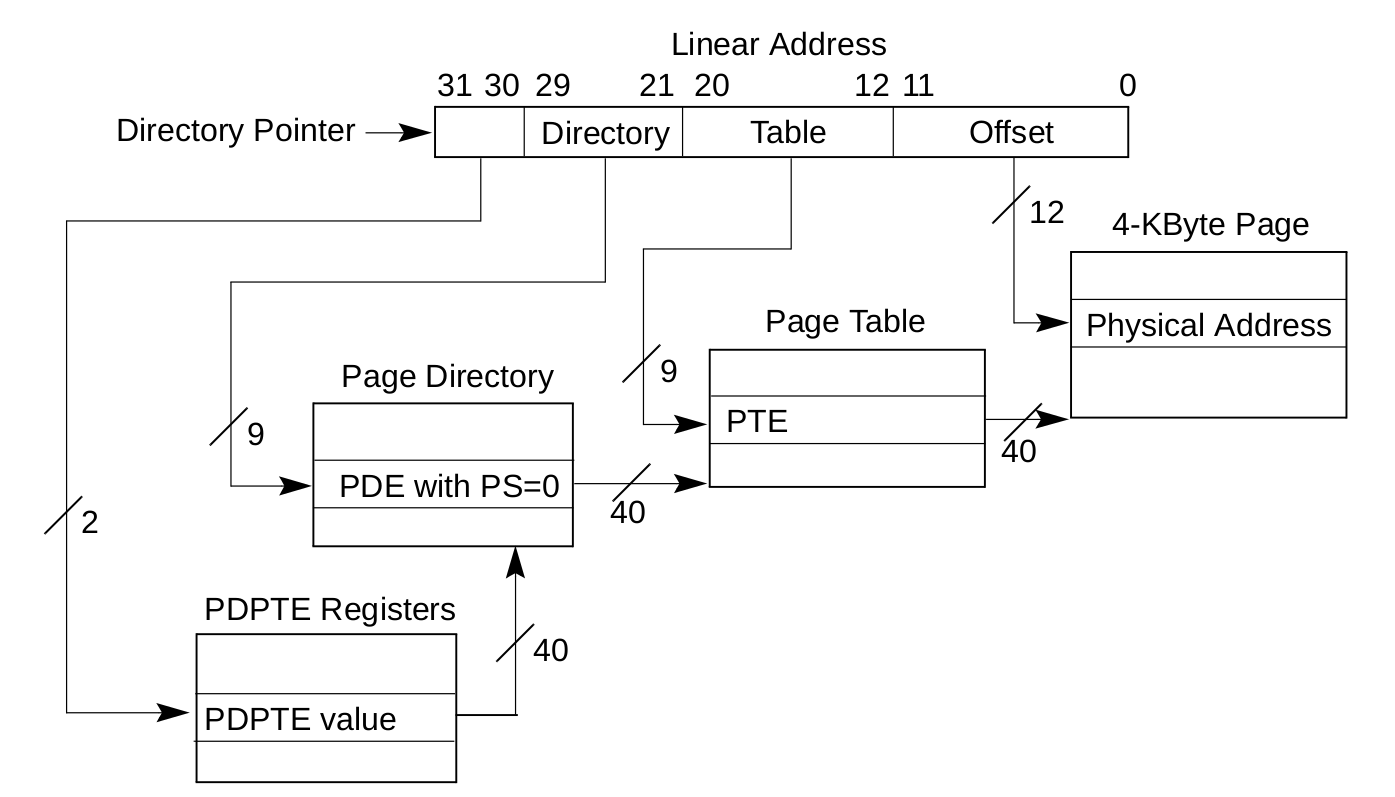
\includegraphics[width=0.8\textwidth]{pae.png}
  \fig{6}{0 pt}{PAE Paging (\cite{intel} pp. 114) }
\end{center}

Since the amount of RAM \marginnote{In order to enable PAE bit 5 of \texttt{CR4} must be asserted} supported by a processor is limited by the number of address pins connected to the address bus this means that 32-bit processors can physically address only up to 4GB of RAM in theory. The increasing need of memory in big servers created a pressure on Intel to expand the amount of RAM supported by this architecture. Intel satisfied these requests by increasing the number of address pins on its processors from 32 to 36 bits. This allowed up to $2^{36}$ = 64GB of RAM and reduced the amount of swap.

To \marginnote{(\cite{bovet_cesati_2006} pp. 52)} support PAE the paging mechanism was changed with the one shown in Figure 3.6 moving to a three level paging:

\begin{itemize}
  \itemsep-3pt
  \item PTE Address field was extended from 20 bits to 24 meaning that the 64GB of memory are split into $2^{24}$ distinct page frames ($2^{24} \times$ 4KB = 64GB). Since the Address field has increased in size and the 12 flag bits described above are still included the PTE size is doubled to 8 bytes (24 + 12 = 36 bits are needed) therefore 4KB/8B = 512 entries fit in one PT/PD page (9 bits used to index the PTE/PDE in the Linear Address, $2^9 = 512$).
  \item A new first level of page table called Page Directory Pointer Table (PDPT) consisting of four 8 byte entries has been introduced (2 most significant bits of the Linear Address for indexing the PDPTE, $2^2$ = 4 entries)
  \item PDPTs are required to be stored in the first 4GB of RAM and aligned to a multiple of $2^5 = 32$ bytes (4 entries $\times$ 8 bytes). Through this scheme only 27 bits of \texttt{CR3} are used to store the physical address of the PDPT ($2^{27} \times 2^5 = 2^{32} = $ 4GB)
  \item Once \texttt{CR3} is set still only 4GB of RAM can be addressed ($2^2 \times 2^9 \times 2^9 \times 2^{12} = 2^{32}$) and changing \texttt{CR3} for some process can be difficult since same Linear Addresses must be used in different pieces of code. 
\end{itemize}

Similarly to the previous addressing scheme PAE allows big pages to be allocated at PD level. 

\subsection{x64, long addressing scheme (IA-32e)}

Moving from 32-bit to 64-bit processor the Logical Address Space increases exponentially and new mechanisms must be introduced to improve paging. Considering that $2^{64}$ Bytes of RAM are unimaginable, Intel decided to shortcircuit bits \texttt{[63:48]} to the same value of bit 47. This splits the Logical Address space into three parts:
\begin{itemize}
  \itemsep-3pt
  \item Canonical "lower half": addressable addresses from \texttt{0x0} to \texttt{0x00007FFF FFFFFFFF}
  \item Noncanonical addresses: unaddressable memory from the previous address to \texttt{0xFFFF8000 00000000}
  \item Canonical "higher half": addressable addresses from the previous to \texttt{0xFFFFFFFF FFFFFFFF}
\end{itemize}

Theoretically a total of 256TB of memory is addressable. 

In terms of page table organization we move from a three level page table in PAE to a 4 level page table in long mode introducing the Page Manager Level 4 (PML4 or also called Page General Director (PGD) ) table. PTE size is still 8 Bytes but 36 bits are used for the Address field. The scheme is the similar to PAE but in this case also 1GB pages (Huge Pages) can be directly mapped through a PDPTE. 

\marginnote{In Linux the canonical higher half is reserved for the kernel while the canonical lower half for user-space as shown in the \href{https://www.kernel.org/doc/Documentation/x86/x86_64/mm.txt}{documentation}.}

\begin{center}
  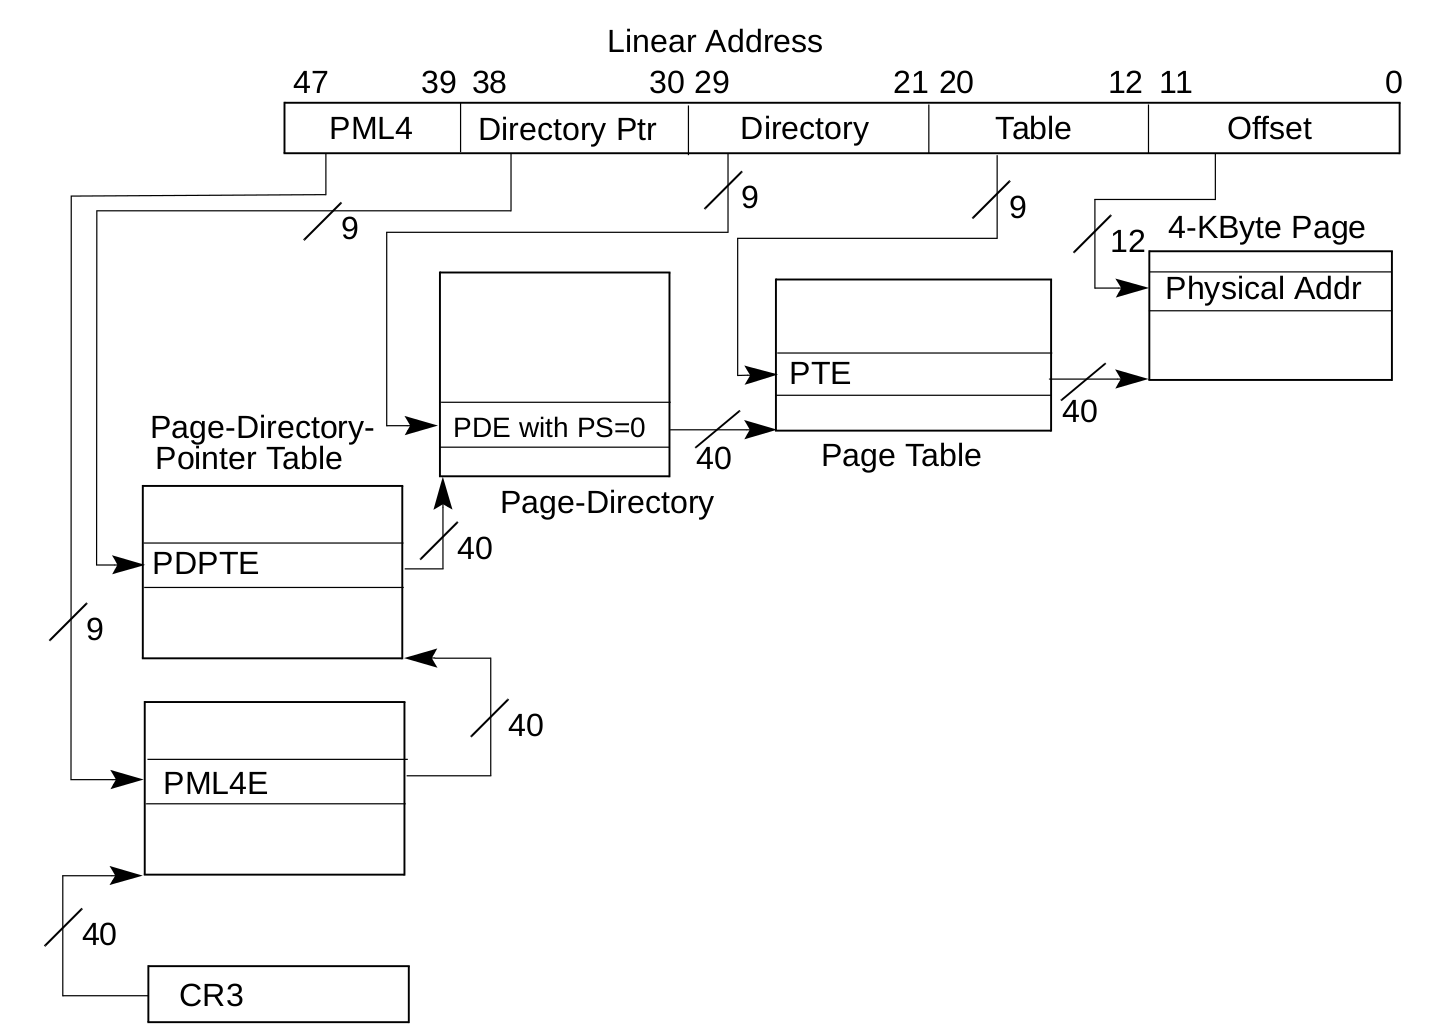
\includegraphics[width=0.8\textwidth]{x64pag.png}
  \fig{7}{0 pt}{IA-32e Paging (\cite{intel} pp. 124) }
\end{center}

\section{Translation Lookaside Buffer}

Since the translation of addresses require multiple accesses to memory for reading the page tables, 80x86 processors include another cache besides other general-purpose hardware caches specifically for speeding up address translation called Translation Lookaside Buffer (TLB).

As we saw previously a Linear Address is splitted into multiple parts. The upper bits of a Linear Address (called the \textbf{page number}) determine the upper bits of the Physical Address (called \textbf{page frame}) through a "walk" in the page tables; the lower bits (called \textbf{page offset}) correspond to the lower bits of the Physical Address.

The \marginnote{(\cite{intel} pp. 140)} TLB caches the mapping of Linear Addresses to Physical Addresses by keeping several entries corresponding to individual translations. The TLB's entries are referenced through the page number of the address that needs to be translated and contain the Physical Address of the page frame corresponding to that Linear Address.

In \marginnote{There is one TLB per core} this scenario the MMU may not consult the page tables for translating a Linear Address for which a TLB entry is present speeding up the translation process. In case of TLB miss (no entry being present for a given Linear Address) the firmware consults the paging structures to obtain the Physical Address which is then cached in the TLB for future translations.  

In \marginnote{(\cite{intel} Sec. 4.12)} the case of the requested Linear Address not having a Physical Page mapped to it (Present bit clear) a page fault exception is generated. The handler for page-fault exceptions typically directs the operating system or executive to load data for the unmapped page from external storage into physical memory (perhaps writing a different page from physical memory out to external storage in the process) and to map it using paging (by updating the paging structures). When the page has been loaded into physical memory, a return from the exception handler causes the instruction that generated the exception to be restarted. \marginnote{\textcolor{red}{(\cite{bovet_cesati_2006} pp. 142) For hardware handling to be added on Lec2 when checking privileges}}

\iffalse
What we would like to end up in is having the kernel on the upper side of memory (1GB) and the remainder memory used for User Space. We're talking about virtual memory. The kernel knows the first address of its virtual memory it is using and where it is loaded in physical memory and with these informations performs the translation. It maps itself contiguously in memory.

\subsection{Linux memory layout}

A bunch of addresses that cannot be used and the kernel puts itself below the non canonical part. Software is put in the higher part of the memory. The lower portion is used for stack, heap, shared objects etc. The kernel is not put in the lower part since in this way you can always increase the size of the kernel without remapping anything about the internal organization of the kernel.

\section{Page table in x64}

In the linear address there are 48 bits. If 64 bits were used instead of that the page table would have to grow too much. The 4th level introduced is PML4 Page Manager Level 4. PML4 is also called Page General Directory (PGD). Each table fits within a page. 

CR3 didn't change much except for the size. The presence bit set to 0 ignores everything of a portion in the entry. Linux uses this part to store where the page is stored in secondary storage. Huge pages are also introduced to have 1GB pages. Motivation: used for hypervisors and virtualization to map large files. qemu uses huge pages.

These new facilities need to be enabled as well.
\fi

\section{Enabling x64 longmode}

The code for enabling x64 longmode is the following

\begin{verbatim}
  movl $MSR_EFER, %ecx            ; read Model Specific Register 0xC0000080
  rdmsr                           ; content is written in edx:eax
  btsl $_EFER_LME, %eax           ; set bit 8 to enable long mode
  wrmsr                           ; write MSR

  pushl $__KERNEL_CS              ; push Code Segment Selector for lret
  leal startup_64(%ebp), %eax     ; dyn calculate jump address
  pushl %eax                      ; push return address for lret

  movl $(X86_CR0_PG | X86_CR0_PE), %eax
  movl %eax, %cr0                 ; enable paging, set PE and PG in CR0
  lret 
\end{verbatim}

Before doing so, various data structures and configurations must be performed as described in the Intel manual (\cite{intel} pp. 323). 

\marginnote{MSR are Intel's specific registers for debugging purposes. One of these registers was then used to adopt AMD's longmode introduced with the EFER register}[-2cm]

\iffalse
\section{Huge Pages}

Linux doesn't have software facilities for mapping real huge pages. Memory advise.
https://www.kernel.org/doc/Documentation/vm/hugetlbpage.txt
\fi


\section{Linux Boot in i386 ($<$ v. 2.6)}

By Stage 1 Bootloader is meant the code held in the MBR (bootsector present in the first sector of the disk). In the early i386 version of Linux a \textit{boot sector} that ran in 16-bit real mode was implemented to perform BIOS boot which is available at \texttt{arch/i386/boot/bootsect.S} acting as a Stage 1 Bootloader. This piece of code moved itself from \texttt{0x07C0} (which is the address where the BIOS had loaded it) to \texttt{0x90000}, read the disk and loaded into memory \texttt{arch/i386/boot/setup.S}.

The \marginnote{ (\cite{bovet_cesati_2006} pp. 838, referring to \texttt{setup.S})} latter code was responsible for getting the system data from the BIOS, and putting them into the appropriate places in system memory (\texttt{start_of_setup}) plus other system configuration. It read the physical memory map through the E820 BIOS facility, enabled the A20 line, setup a temporary IDT and GDT, performed the switch to 32-bit \textbf{protected mode} and finally loaded the compressed image of the kernel and gave control to the function \texttt{startup_32} in \texttt{arch/i386/\textcolor{red}{boot/compressed}/head.S}.

The \texttt{startup_32} function decompressed the kernel image and jumped to another function having the same name (\texttt{startup_32}) in \texttt{arch/i386/\textcolor{red}{kernel}/head.S} which enabled paging and setup again the GDT and IDT (temporarily ignoring all interrupts).

Later in time new bootloaders came along such as LILO and GRUB acting as Stage 1 and Stage 2 Bootloaders able to navigate the file system, start up a boot selection menu by reading a configuration file and load the selected OS image.

\section{UEFI}

The primary goal of the UEFI specification is to define an alternative boot environment that can alleviate firmware developers from crafting complex solutions for being compatible with new hardware specifications and platform capabilities.

UEFI firmware is capable of executing UEFI executables which are regular Portable Executable (PE) images runnable under various platforms containing multiple services such as bus, block, file services, graphical consoles and booting over network. Various libraries exist to write UEFI applications which run during the pre-boot phase. A virtual machine specification based on a byte code format called EFI Byte Code (EBC) which can be used to write platform-independent device drivers is included in UEFI.

A legacy BIOS loads a 512 byte flat binary blob from the MBR of the boot device into memory at physical address \texttt{0x7C00} and jumps to it. The bootloader cannot return back to BIOS. UEFI firmware loads an arbitrary sized UEFI application from a FAT partition called EFI System Partition (ESP) on a GPT-partitioned boot device to some address selected at run-time. Then it calls that application's main entry point. The application can return control to the firmware, which will continue searching for another boot device or bring up a diagnostic menu. The boot configuration is defined by variables stored in NVRAM, including variables that indicate the file system paths to OS loaders and OS kernels. UEFI boot targets can be found under \texttt{/efi/boot/}.

\subsection{GUID Partition Table}

One of the main drawbacks of BIOS was the 32-bit addressing scheme of partitions that allowed only to point to at most 512B $\times 2^{32} =$ 2TB (512B is the size of a sector) within a disk. Clearly this became a problem with Hard Disk sizes growing over-time constraining the partition scheme of large disks.

In UEFI the problem is addressed by using GUID Partition Table scheme instead of MBR. For limited backward compatibility, the space of the legacy MBR is still reserved in the GPT specification, but it is now used in a way that prevents MBR-based disk utilities from misrecognizing and possibly overwriting GPT disks.

The partition table header defines the usable blocks on the disk. It also defines the number and size of the partition entries that make up the partition table.

\marginnote{
  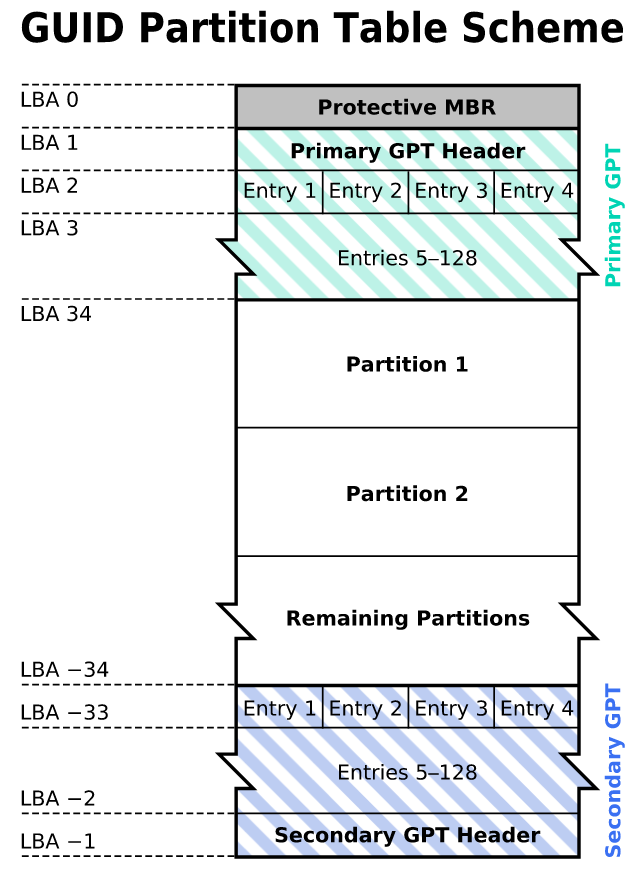
\includegraphics[width=0.4\textwidth]{gpt.png}
  \fig{8}{0 pt}{GUID Partition Table Scheme \cite{gpt}}
}[-7cm]

After the header, the Partition Entry Array describes partitions, using a minimum size of 128 bytes for each entry block. The starting location of the array on disk, and the size of each entry, are given in the GPT header. The first 16 bytes of each entry designate the partition \textit{type}'s globally unique identifier (GUID). For example, the GUID for an EFI System Partition is \texttt{C12A7328-F81F-11D2-BA4B-00A0C93EC93B}. The second 16 bytes are a GUID unique to the partition. Then follow the starting and ending 64 bit addresses, partition attributes, and the Unicode partition name.

Finally a copy of the Primary GPT, namely Secondary GPT, is kept at the end of the disk for backup purposes.  

\subsection{Secure Boot}

Another \marginnote{\cite{kumar_kumar_2007}} issue with the BIOS interface was the spread of malwares that infected the MBR (Bootkits). One example of such malwares is Vboot Kit. An hard disk is infected by overwriting the content of its MBR with the code of the rootkit and relocating the old bootloader in another portion of the hard disk.

On system startup the BIOS loads the MBR (and therefore the rootkit's code) into memory and jumps into its address. Vboot Kit hijacks \texttt{int 0x13} in the IVT by replacing the BIOS services for reading and writing the hard disk with its own hooks and then loads the bootloader.

When the bootloader will trigger \texttt{int 0x13} to ask the BIOS to read some data from the hard disk the Vboot Kit hook will execute and patch the code segments that were asked to be loaded and will gain control of the system.

Secure \marginnote{(\cite{secb} pp. 7)} Boot mitigates such attacks ensuring that UEFI firmware will load only signed executables. A series of asymmetric keys and databases are used to manage and protect the  signatures needed  to verify code before it is executed.

First, there is the \textbf{Platform Key (PK)}. This key is typically set by the platform manufacturer when a system  is built in the factory. While it may be replaceable by an end user or enterprise IT services, its purpose is to protect the next key from uncontrolled modification \cite{PK}.

The second key is the \textbf{Key Exchange Key (KEK)}, which protects the \textbf{Signature Datab}- \textbf{ase} from unauthorized modifications. No changes can be made to the signature database without the private portion of this key. There can be multiple KEKs provided by the operating system and other trusted third party application vendors. A holder of a valid KEK can insert or delete signatures in a signature database. The database maintains two lists of signatures: signatures of code that is authorized to run on the platform and signatures of code that is forbidden. 

When loading the operating system bootloader the firmware confirms that its signature matches one in its database of authorized signatures, and also that the signature is not in the forbidden database.

\section{Multicore Booting}

As \marginnote{(\cite{intel} Sec. 8.4)} anticipated in Lecture 1 following a power-up or RESET of an Multi Processor (MP) system an Hardware MP initialization protocol is run to select the Boostrap Processor (BSP) and the Application Processors (APs). The BSP is the one executing BIOS and all the other code of system initialization while APs wait for a specific signal from the BSP.

To perform \marginnote{(\cite{intel} Chap. 10)} sophisticated interrupt sending and redirection Intel introduced the Advanced Programmable Interrupt Controller (APIC).  The APIC interface is composed of two parts: a local APIC for each logical processor and an external I/O APIC part of the system's chipset.

The local APIC has multiple registers for various kinds of operations all memory mapped to a 4KB page frame with initial starting address \texttt{0xFEE00000}. Within them can be found the Interrupt Command Register (ICR) which allows software running on some processor to send Interprocessor Interrupts (IPIs) to other processors. Two pins are connected to the processor from the local APIC: \texttt{LINT0} and \texttt{LINT1}, the former being normal interrupts and the latter non-maskable interrupts.

In order for the APs to start executing code the BSP must send the INIT-SIPI signal to them through the ICR and this is done by writing the lower 32 bits out of the 64 of the address (\texttt{0xFEE00300}) mapped to the ICR.

\marginnote{(\cite{intel} pp. 278}

\begin{verbatim}
        mov $sel_fs, %ax
        mov %ax, %fs
        
        ; send INIT to all-except-self
        mov $0x000C4500, %eax
        mov %eax, %fs:(0xFEE00300) 11 00 0 1 0 0 0 101 00000000

.B0:    btl $12, %fs:(0xFEE00300)
        jc .B0
        
        ; send SIPI to all-except-self
        mov $0x000C4611, %eax
        mov %eax, %fs:(0xFEE00300) 11 00 0 1 0 0 0 110 00010001

.B1:    btl $12, %fs:(0xFEE00300)
        jc  .B1
\end{verbatim}

\begin{center}
  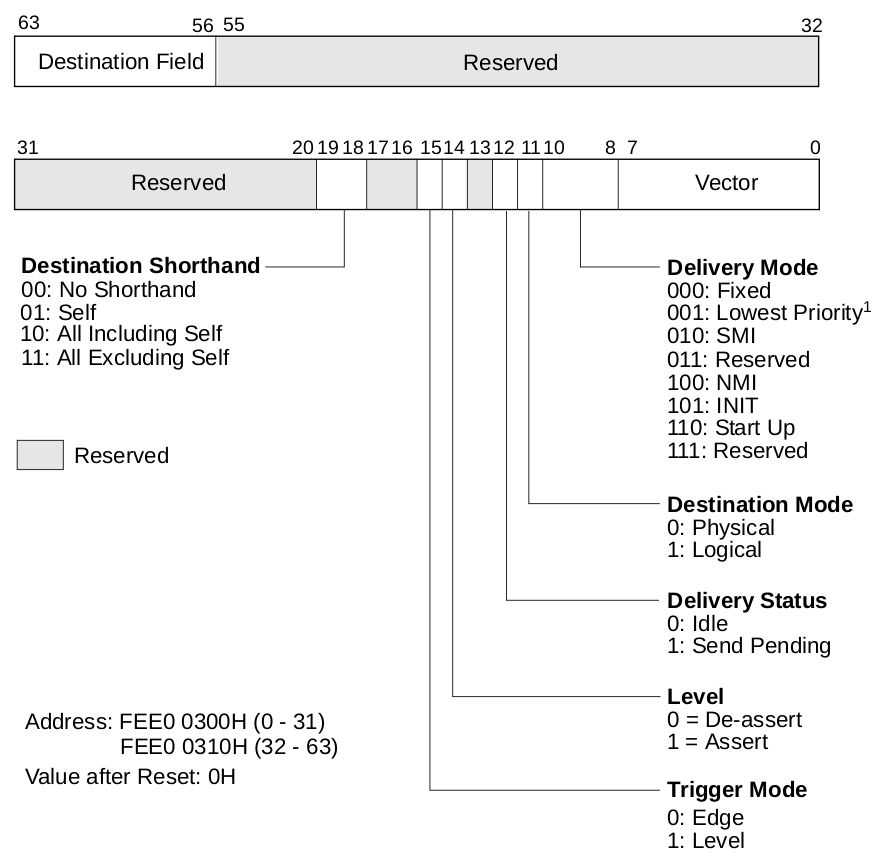
\includegraphics[width=0.6\textwidth]{icr.png}
  \fig{9}{0 pt}{ICR bit interpretation (\cite{intel} pp. 381) }
\end{center}

The Vector field determines the real-mode base address of the 4-KByte page for the APs' boot code which must reside in the first megabyte of memory ($2^{8} \times 4$KB = 1MB). Therefore the address for the example shown above is \texttt{0x11000}. Interrupts can be sent either specifying a cpu lAPIC id through the Destination field or through the Destination Shorthand (bit 19 and 18). In both INIT and SIPI the destination shorthand is used since the interrupt must be sent to all
the APs.

\textcolor{red}{FS register usage for indicating right register (?)}

\newpage
\bibliography{Lec3}
\bibliographystyle{plainnat}
\end{document}
